\section{Operator}
\label{sec:komponenten:operator}

Operatoren, auch Controller genannt, bieten die Möglichkeit, die Kubernetes API mit eigenen Objekten und Funktionen zu erweitern.

\begin{figure}[h]
  \centering
  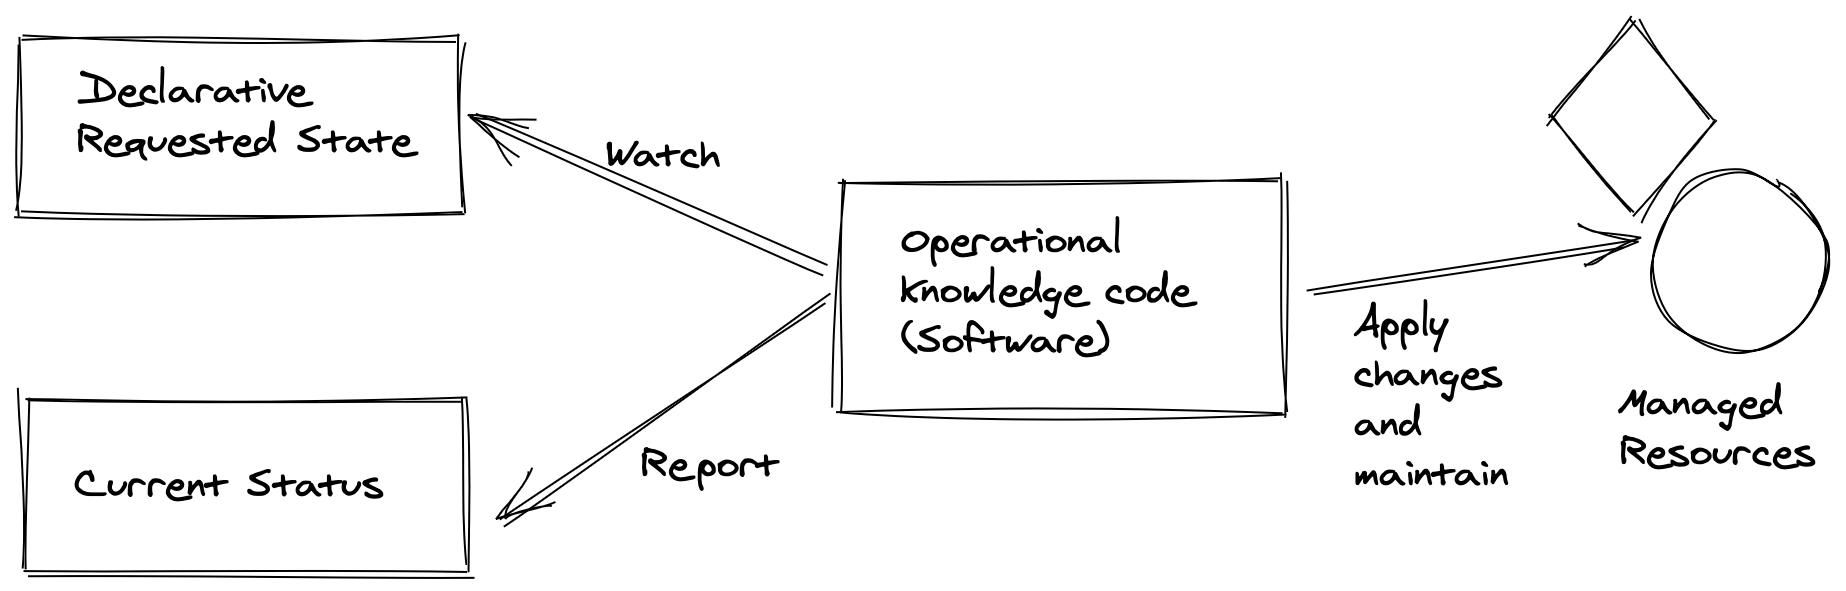
\includegraphics[width=\textwidth]{gfx/chapters/3_komponenten/operator_highlevel.png}
  \caption{High Level Überblick von Operatoren}
  \label{fig:kubernetes_operator_highlevel}
  \source{\cite{operatorWhitepaper}}
\end{figure}

Zur Verdeutlichung zeigt Abbildung \ref{fig:kubernetes_operator_highlevel} einen abstrakten Überblick zu Operatoren. 
Durch Nutzen eines Operators befindet sich jegliches Wissen zum Anpassen und Verwalten eines Objekts im Programmcode \cite{operatorWhitepaper}.

\begin{figure}[h]
  \centering
  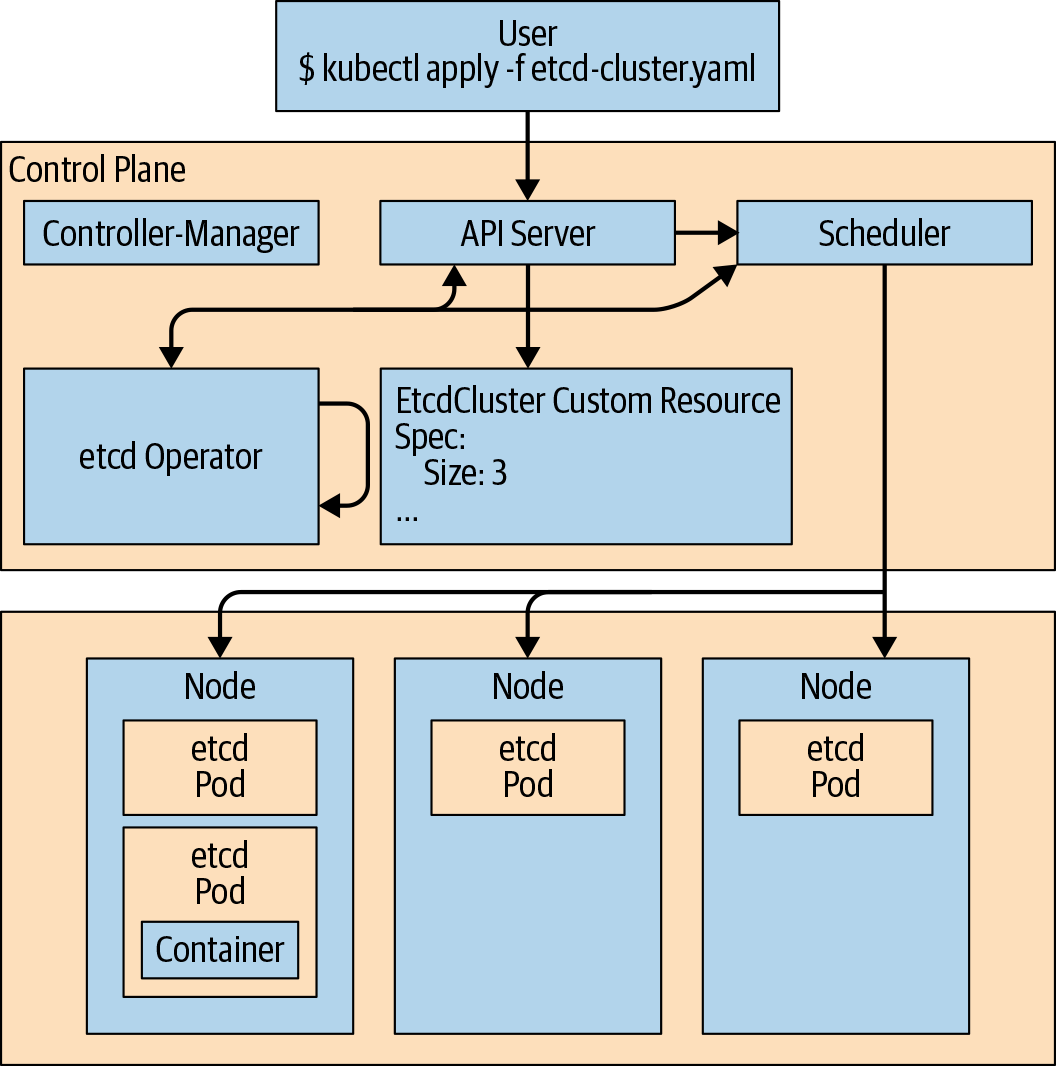
\includegraphics[width=0.8\textwidth]{gfx/chapters/3_komponenten/operator_example.png}
  \caption{Funktionen eines Kubernetes Operators}
  \label{fig:kubernetes_operator_example}
  \source{\cite{Dobies2020}}
\end{figure}

In Abbildung \ref{fig:kubernetes_operator_example} wird die Kommunikation des Operator im Cluster dargestellt.
Der Operator überwacht den API-Server auf Änderungen seiner zugewiesenen \ac{CR} Objekte.
Auf Grundlage des Zustands der Objekte im Cluster ergreift er erforderliche Maßnahmen zur Erfüllung des gewünschten Zustands,
wie beispielsweise das Erstellen neuer Pods \cite{Dobies2020}.
Diesen Synchronisationsmechanismus nennt man \emph{Reconciliation}.

Der für diese Referenzimplementation eines Chat \ac{SaaS} entwickelte Operator nutzt diesen Synchronisationsmechanismus,
um die Erstellung der Rocket.Chat Instanz zu vereinfachen.
Der Rocket API Server erstellt ein Rocket Objekt im Cluster und überlässt jegliche Verwaltung der eigentlichen Instanz dem Operator.
Operatoren können sich zusätzlich zur Bereitstellung und Konfiguration der Anwendung auch um die Funktionen Backup
und automatische Reparatur des Services kümmern \cite{Dobies2020}.
Zur Einhaltung von validen Schemas des Objekts (siehe \ref{subsection:kubernetes:customresource}),
wie beispielsweise die Nutzung eines existierenden Container Images für den Rocket Webserver,
kann ein \emph{Admission Controller} genutzt werden.
Die Funktion zur Erstellung von Backups sowie der Validierung durch einen Admission Controller
wurden allerdings in dieser Referenzimplementation nicht berücksichtigt wurden.


Eine Rocket.Chat Instanz besteht aus einer MongoDB, welche als Replicaset konfiguriert wird,
sowie dem eigentlichen Webserver, der als Endpunkt für Rockets Clientsoftware dient \cite{rocketChatDocs}.
Für die Bereitstellung eienr Chat Instanz werden die folgenden Kubernetes Objekte im Cluster angelegt:
\begin{itemize}
  \item ConfigMap für MongoDB Scripts
  \item Secret für MongoDB Authentifizierung (Nutzername und Passwort)
  \item \ac{PV} für MongoDB
  \item Service für Webserver und MongoDB Pods
  \item Deployment für Webserver Pods
  \item StatefulSet für MongoDB Pods
  \item Ingress für Webserver
  \item ServiceAccount
\end{itemize}

\newpage
\subsection{Rocket Custom Resource}
Als Schnittstelle für Kommunikation mit dem Operator dient das Rocket \ac{CR} Objekt.
Dies wird im Code als nativer Datentyp definiert und schließlich zu einem \ac{CRD} generiert, um es im Kubernetes Cluster zu installieren.
Genauer dargestellt wird die Spezifikation des Objekts in \ref{chap:rocketchat_crd_spec}.
Nutzer des Kubernetes Cluster können selbst Rocket \acp{CR} Objekte via YAML oder JSON Dateien erstellen und
an die Kubernetes API schicken. Dieser Anwendungsfall ist für Kunden allerdings nicht vorgesehen.
Endnutzer sollen sich nicht mit der Komplexität von Kubernetes auseinander setzen müssen,
sondern nur per Konfiguratorclient (\ac{CLI} oder Webinterface) ihren Chat Service erstellen.


